\chapter{Evaluation}

In the previous chapters, we present the design of the SableWasm compiler and runtime. This chapter will focus on the performance evaluation in terms of the execution speed of the generated shared libraries. Here, we focus on three research problems. First, how does SableWasm performs compares to other WebAssembly runtime environment implementations? Second, does the optimization over the input WebAssembly module affect the overall performance? Finally, how much does the WebAssembly SIMD extension improve comparing to optimized scalar counterparts? We will first present the setup for experiments used when investigating three questions, and later, the experiment results for each one of them.

\section{Experiment Setup}

This section presents the setup for the experiments in the remaining part of the chapter. We conduct the benchmarks on the same server for all experiments. The server has a The experiments were performed on a six-core Intel Core processor at a 3.7 GHz standard clock frequency and an L3 cache of 12 MiB. Additionally, The server runs Ubuntu 18.04 with Linux kernel version 4.15.0 and 32GiB of memory. When measuring the performance, we execute each benchmark ten times in succession to minimize the measurement error as some of the benchmarks take less than a second to complete. Finally, the final benchmark result is the average among ten runs except the highest and the lowest. For the benchmark subject, we choose three different benchmark suits, the Polyhedral benchmark suite (Polybench), the Ostrich benchmark suite (Ostrich) and the NAS parallel benchmarks (NPB).

\begin{table}
    \centering
    \begin{tabular}{|l|l|}
        \hline
        \textbf{Benchmark Name} & \textbf{Description}                                \\ \hline
        2mm                     & 2 matrix multiplication (D = A.B; E = C.D)          \\ \hline
        3mm                     & 3 matrix multiplication (E = A.B; F = C.D; G = E.F) \\ \hline
        adi                     & alternating direction implicit solver               \\ \hline
        atax                    & matrix transpose followed by vector multiplication  \\ \hline
        bicg                    & BiCG sub kernel of BiCGStab linear solver           \\ \hline
        cholesky                & Cholesky decomposition                              \\ \hline
        correlation             & correlation computation                             \\ \hline
        covariance              & covariance computation                              \\ \hline
        doitgen                 & multiresolution analysis kernel (MADNESS)           \\ \hline
        dynprog                 & dynamic programming (2D)                            \\ \hline
        fdtd-2d                 & 2D finite different time domain kernel              \\ \hline
        fdtd-apml               & FDTD using anisotropic perfectly matched layer      \\ \hline
        gauss-filter            & gaussian filter                                     \\ \hline
        gemm                    & matrix-multiply (C = alpha.A.B + beta.C)            \\ \hline
        gramschmidt             & Gram-Schmidt decomposition                          \\ \hline
        jacobi-1D               & 1D Jacobi stencil computation                       \\ \hline
        jacobi-2D               & 2D Jacobi stencil computation                       \\ \hline
        lu                      & LU decomposition                                    \\ \hline
        ludcmp                  & LU decomposition (different implementation)         \\ \hline
        mvt                     & matrix vector product and transpose                 \\ \hline
        reg-detect              & 2D image processing                                 \\ \hline
        seidel                  & 2D Seidel stencil computation                       \\ \hline
        symm                    & symmetric matrix multiplication                     \\ \hline
        syr2k                   & symmetric rank-2k operations                        \\ \hline
        syrk                    & symmetric rank-k operations                         \\ \hline
        trisolv                 & triangular solver                                   \\ \hline
        trmm                    & triangular matrix multiplication                    \\ \hline
    \end{tabular}
    \caption{the Polyhedral benchmark suite (Polybench)}
    \label{tbl:polybench}
\end{table}

\paragraph{Polybench}
The Polyhedral benchmark suite (Polybench) \cite{polybench} contains a group of small math kernel functions as shown in table~\ref{tbl:polybench}. The description table is adjusted from official Polybench documentation\footnote{Polybench: \url{http://web.cse.ohio-state.edu/~pouchet.2/software/polybench/}}. In the WebAssembly announcement paper \cite{10.1145/3062341.3062363}, the community also chooses Polybench as the evaluation subject. However, one problem is that the Polybench is in C. Therefore, the researchers cross-compile the benchmark using a modified Clang compiler with LLVM WebAssembly backend. However, there is no standardized system interface, such as WASI, proposed by the community when publishing the paper. Hence, the experiment is measured with an external clock, and all features that require system interaction are disabled. On the other hand, when evaluating SableWasm, we use a WASI-enabled Clang compiler \footnote{WASI SDK: \url{https://github.com/WebAssembly/wasi-sdk}} to cross-compile the WebAssembly modules into WebAssembly modules. Each benchmark reports its execution time by issuing syscalls to the runtime environment, which in theory, should yield more accurate results, especially for a just-in-time (JIT) runtime environment.

\begin{table}
    \centering
    \begin{tabular}{|l|l|}
        \hline
        \textbf{Benchmark Name} & \textbf{Description}                                        \\ \hline
        back-prop               & backward propagation in a layered neural network            \\ \hline
        bfs                     & breadth-first search in a randomly generated graph          \\ \hline
        crc                     & CRC error-detecting algorithm                               \\ \hline
        fft                     & fast Fourier transform                                      \\ \hline
        hmm                     & forward-backward algorithm over a hidden Markov model       \\ \hline
        lavamd                  & 3D space particle simulation                                \\ \hline
        lud                     & LU decomposition                                            \\ \hline
        nqueens                 & N-queen problem solver                                      \\ \hline
        nw (needle)             & find optimal alignment of two protein sequences             \\ \hline
        page-rank               & page-rank algorithm to measure the importance of a web site \\ \hline
        spmv                    & sparse matrix multiplication with a vector                  \\ \hline
        srad                    & diffusion method for ultrasonic and radar imaging           \\ \hline
    \end{tabular}
    \caption{the Ostrich benchmark suite (Ostrich)}
    \label{tbl:ostrich}
\end{table}

\paragraph{Ostrich}
The second benchmark suite we used in the Ostrich benchmark suite\cite{ostrich}, illustrated in table~\ref{tbl:ostrich}. Comparing to the Polybench, Ostrich focuses on larger scientific problems instead of computation kernels. Ostrich benchmark suite supports multiple programming languages, such as Javascript and C. Here, we prepare the WebAssembly module similar to the Polybench benchmark suite with a WASI-enable Clang compiler. However, unlike the Polybench benchmark suite, which does not require any modification on the source code, we need to tweak the Ostrich benchmark code due to the limitation of WebAssembly specification. This includes hard-coding the command-line arguments and replacing throwing an exception with calling \texttt{exit} function.

\begin{table}
    \centering
    \begin{tabular}{|l|l|}
        \hline
        \textbf{Benchmark Name} & \textbf{Description}                                 \\ \hline
        IS                      & integer sort (bucket sort)                           \\ \hline
        EP                      & Marsaglia polar method for generating random numbers \\ \hline
        CG                      & estimate the smallest eigenvalue of a SPD matrix     \\ \hline
        MG                      & multi-grid on a sequence of meshes                   \\ \hline
        FT                      & fast Fourier transform                               \\ \hline
        BT                      & block tri-diagonal solver                            \\ \hline
        SP                      & scalar penta-diagonal solver                         \\ \hline
        LU                      & lower-upper solver                                   \\ \hline
    \end{tabular}
    \caption{the NAS parallel benchmark suite (NPB)}
    \label{tbl:npb}
\end{table}

\paragraph{NPB}
The last benchmark suite we selected for evaluating SableWasm is the NAS parallel benchmark suite \cite{npb}, shown in the table~\ref{tbl:npb}. We choose this benchmark because of its parallel nature, as the third research question focuses on the SIMD instruction operations. However, the original NPB benchmark suite is in Fortran, and, at the time of thesis writing, there is no cross-compiler between Fortran and WebAssembly. Hence, we choose an OpenMP variant instead \footnote{NPB OpenMP C: \url{https://github.com/benchmark-subsetting/NPB3.0-omp-C}}. Although the currently WASI-enable Clang does not support OpenMP, we can still cross-compile into WebAssembly, as OpenMP code trivially reduces to C.

This section presents the benchmark environment and test cases for the experiment later in the chapter. One may notice some duplication among three benchmark suites, such as the upper-lower matrix decomposition (LU, ludcmp) and fast Fourier transform (FT, fft). However, we will still treat them as different individual test cases for all of them, as they come with various implementations and may lead to performance differences. Another problem that arises when preparing WebAssembly modules for benchmark suits is that some of the generated modules from the WASI-enabled Clang compiler have unexpected behaviour. In NPB, although the WASI-enabled Clang compile can successfully translate all test cases for all eight benchmark cases, there are two among eight test cases that have different behaviour compare to their native counterparts. For example, the WebAssembly module for the IS benchmark case has memory access out-of-bound for native and optimized translation. Also, the module for EP failed when compiled with the optimization flag enabled in the WASI-enabled Clang compiler. We suspect that some unknown bug in the toolchain may exist as it is still under active development. Another cause for the problem is that the OpenMP implementation may contain non-standard operations that result in undefined behaviour. We also test the generated modules against several other WebAssembly runtime environments, and the result is consistent. The last problem we encounter during benchmark is around WebAssembly SIMD operation extensions. As the extension is still under standardization, most runtime environments only support a subset of all instructions. Hence, when comparing SIMD operations, some of the benchmark results are infeasible. However, we still manage to collect SIMD operation performance data for most of the benchmark cases.

\section[RQ1: How does SableWasm perform compare to others?]{{\large RQ1: How does SableWasm perform compare to others?}}

\begin{figure}
    \centering
    \begin{subfigure}[t]{\textwidth}
        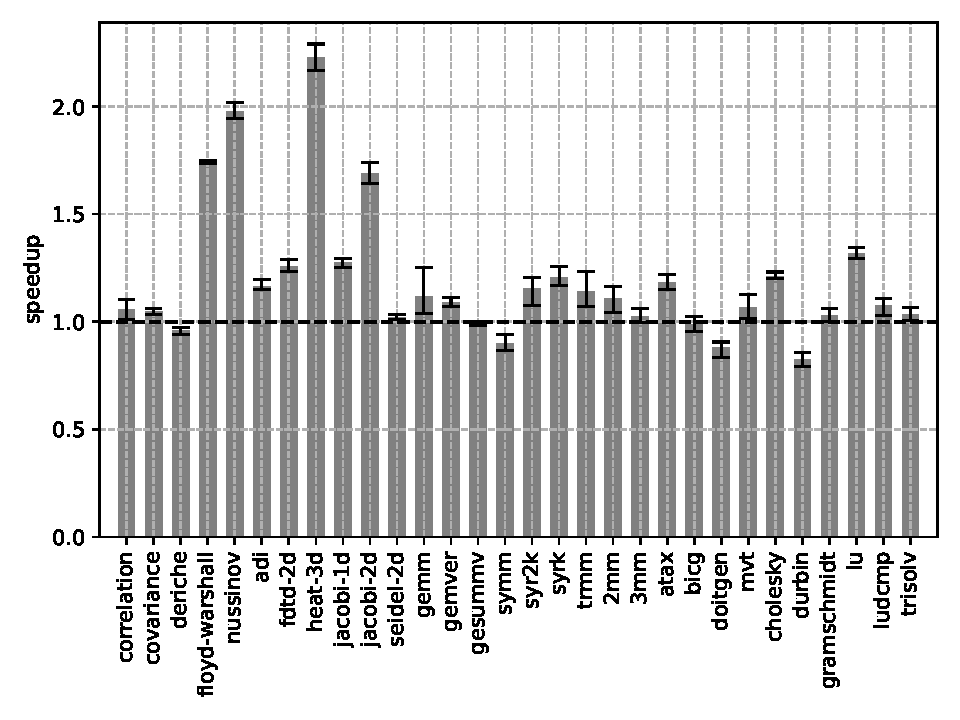
\includegraphics[width=\textwidth]
        {Images/6.1.RQ1/polybench-wasmtime-naive.pdf}
        \caption{Polybench}
    \end{subfigure}
    \begin{subfigure}[t]{.45\textwidth}
        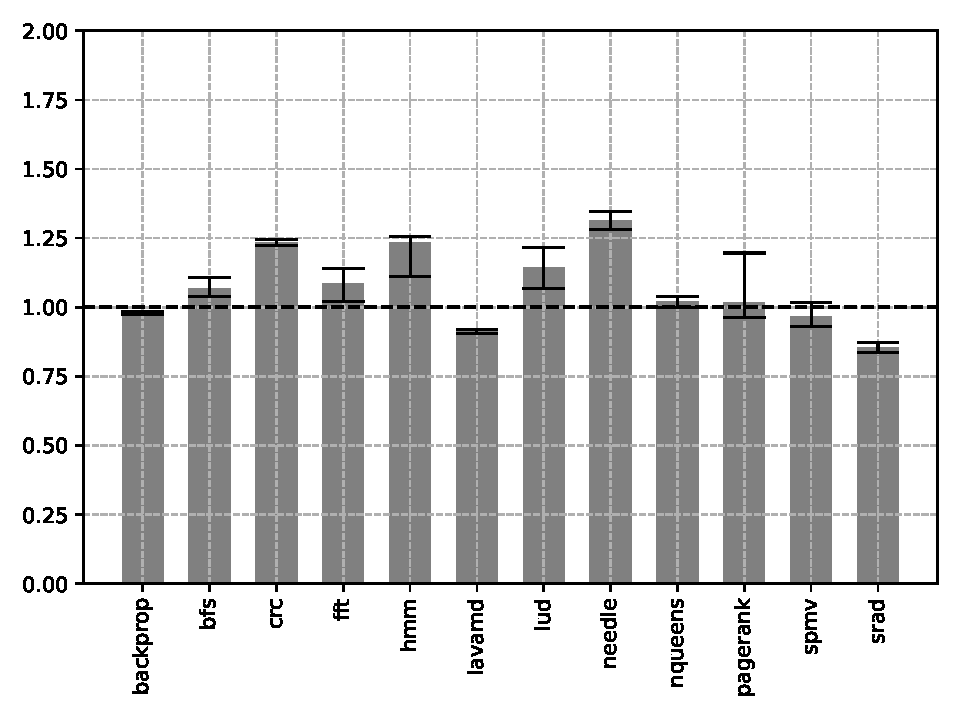
\includegraphics[width=\textwidth]
        {Images/6.1.RQ1/ostrich-wasmtime-naive.pdf}
        \caption{Ostrich}
    \end{subfigure}
    \begin{subfigure}[t]{.45\textwidth}
        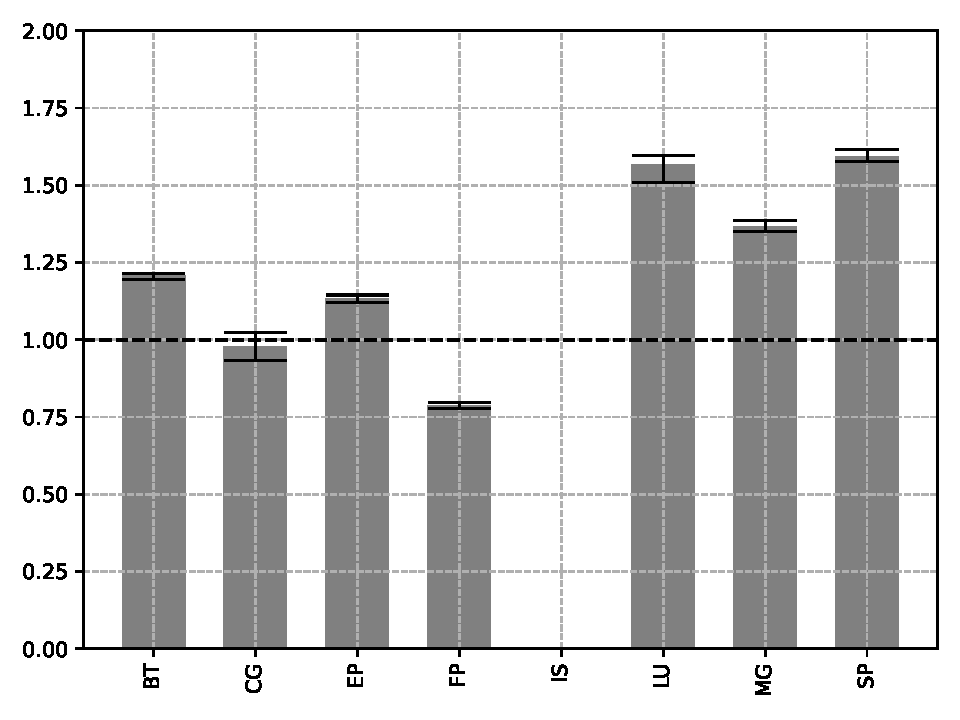
\includegraphics[width=\textwidth]
        {Images/6.1.RQ1/npb-wasmtime-naive.pdf}
        \caption{NPB}
    \end{subfigure}
    \caption{Bechmarks with naive (\texttt{-O0}) on Wasmtime}
    \label{fig:rq1-wasmtime-naive}
\end{figure}

\begin{figure}
    \centering
    \begin{subfigure}[t]{\textwidth}
        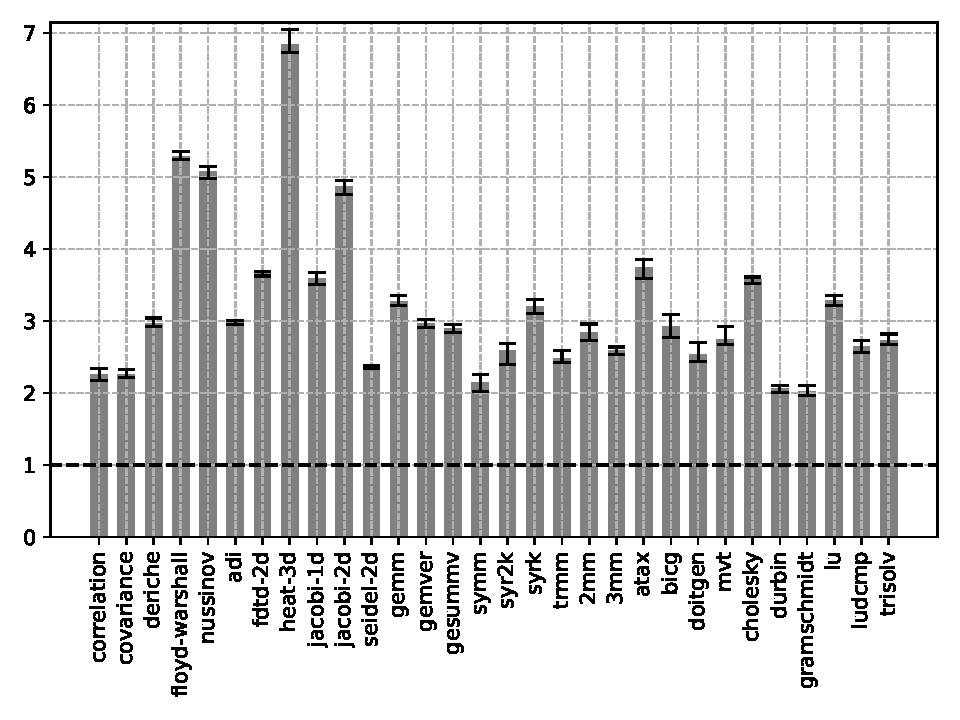
\includegraphics[width=\textwidth]
        {Images/6.1.RQ1/polybench-wasmer-cranelift-naive.pdf}
        \caption{Polybench}
    \end{subfigure}
    \begin{subfigure}[t]{.45\textwidth}
        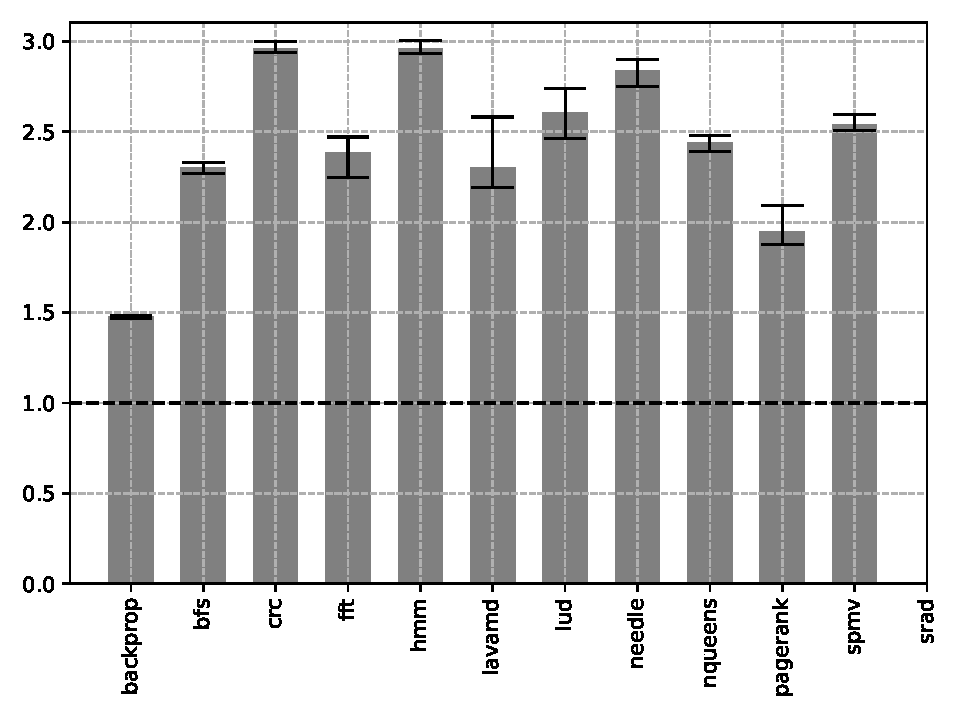
\includegraphics[width=\textwidth]
        {Images/6.1.RQ1/ostrich-wasmer-cranelift-naive.pdf}
        \caption{Ostrich}
    \end{subfigure}
    \begin{subfigure}[t]{.45\textwidth}
        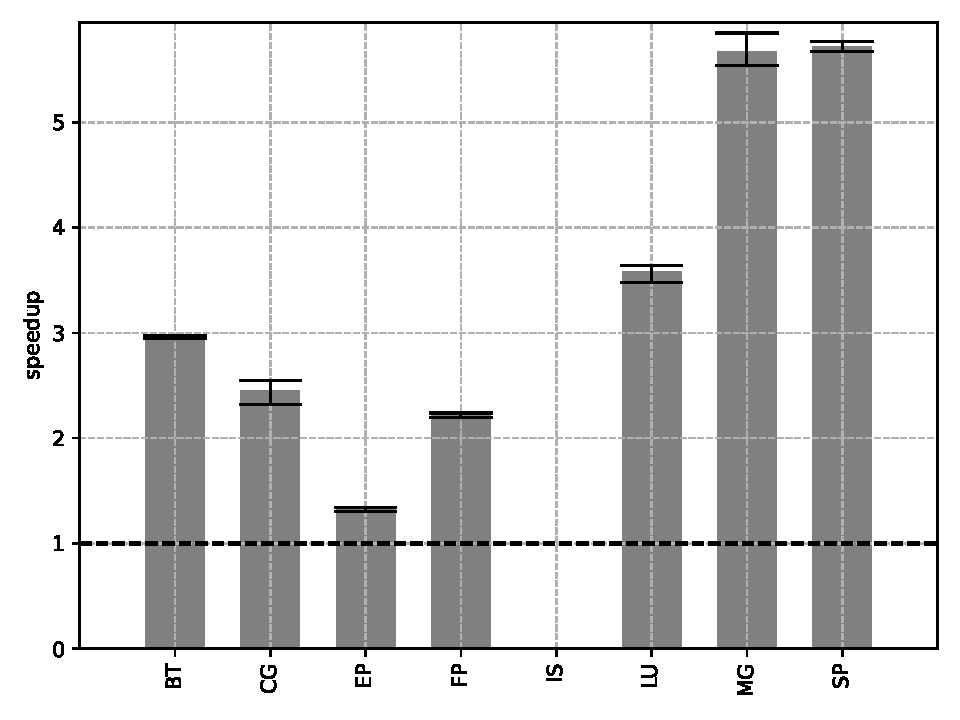
\includegraphics[width=\textwidth]
        {Images/6.1.RQ1/npb-wasmer-cranelift-naive.pdf}
        \caption{NPB}
    \end{subfigure}
    \caption{Bechmarks with naive (\texttt{-O0}) on Wasmer(Cranelift)}
    \label{fig:rq1-wasmer-cranelift-naive}
\end{figure}

\begin{figure}
    \centering
    \begin{subfigure}[t]{\textwidth}
        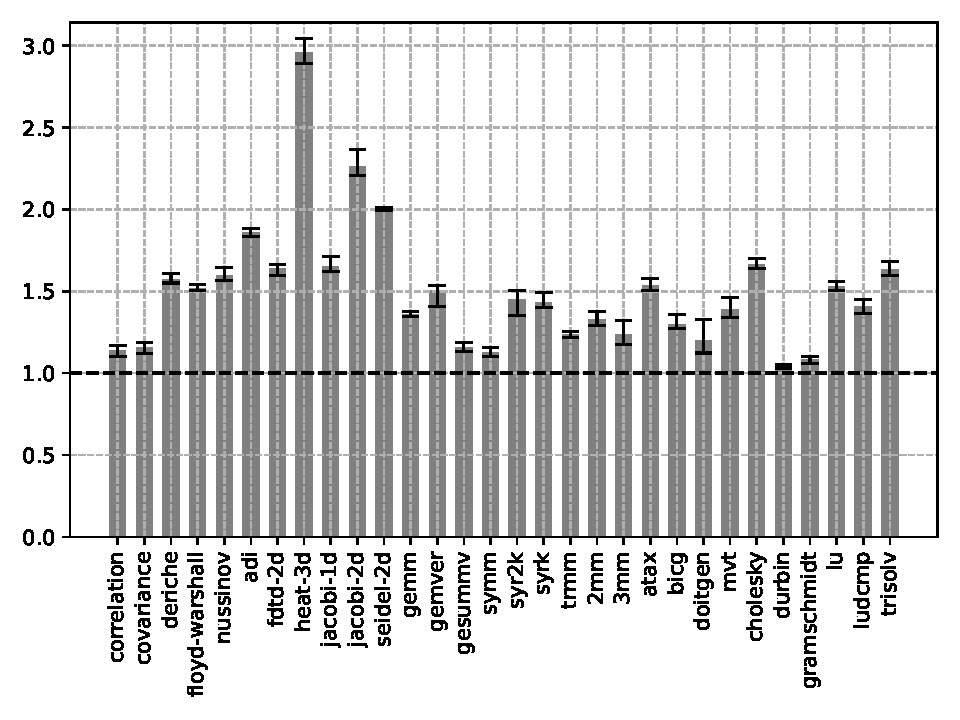
\includegraphics[width=\textwidth]
        {Images/6.1.RQ1/polybench-wasmer-llvm-naive.pdf}
        \caption{Polybench}
    \end{subfigure}
    \begin{subfigure}[t]{.45\textwidth}
        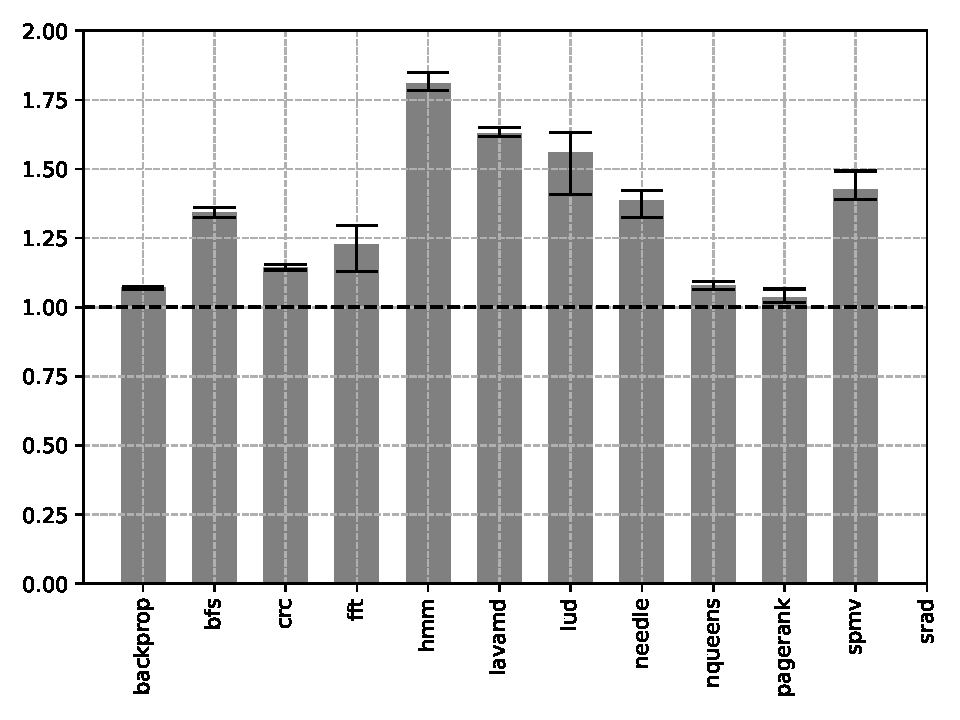
\includegraphics[width=\textwidth]
        {Images/6.1.RQ1/ostrich-wasmer-llvm-naive.pdf}
        \caption{Ostrich}
    \end{subfigure}
    \begin{subfigure}[t]{.45\textwidth}
        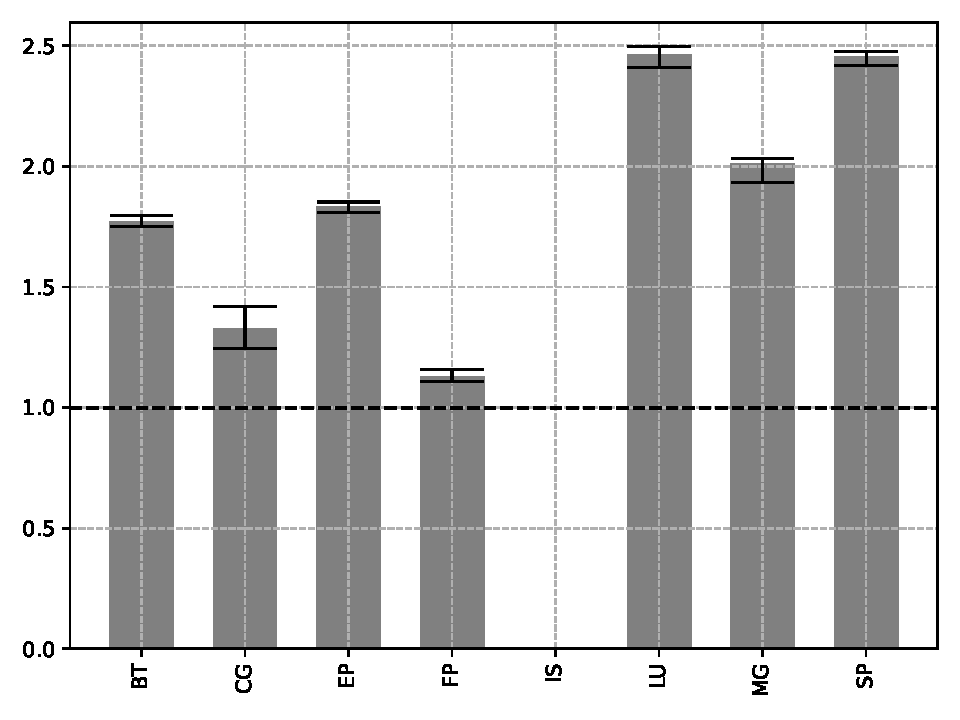
\includegraphics[width=\textwidth]
        {Images/6.1.RQ1/npb-wasmer-llvm-naive.pdf}
        \caption{NPB}
    \end{subfigure}
    \caption{Bechmarks with naive (\texttt{-O0}) on Wasmer(LLVM)}
    \label{fig:rq1-wasmer-llvm-naive}
\end{figure}

\begin{figure}
    \centering
    \begin{subfigure}[t]{\textwidth}
        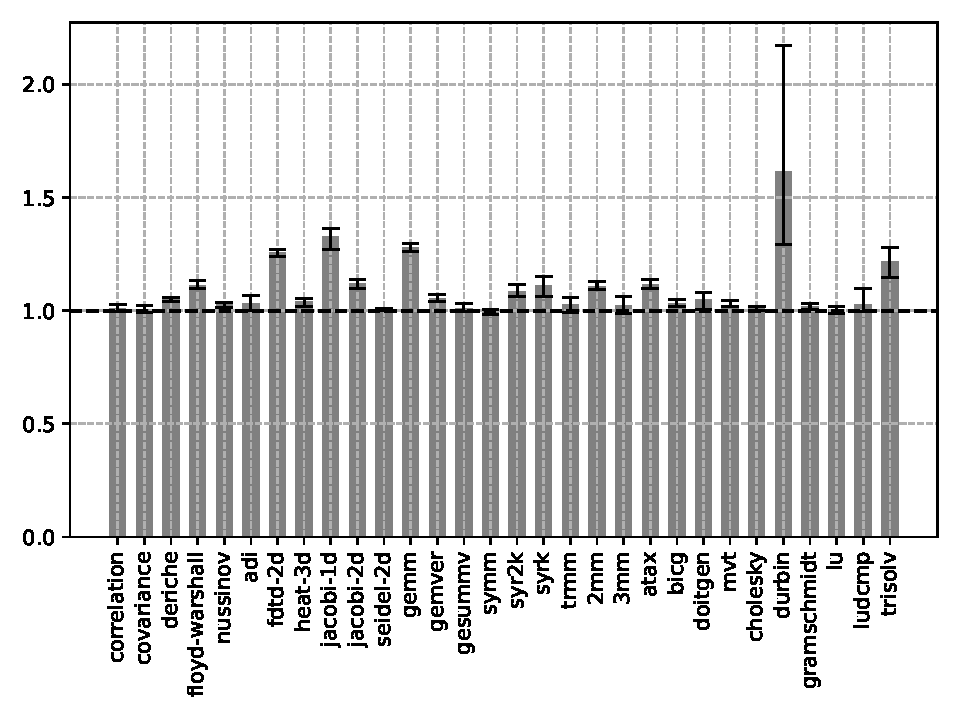
\includegraphics[width=\textwidth]
        {Images/6.1.RQ1/polybench-wasmtime-opt.pdf}
        \caption{Polybench}
        \label{fig:rq1-wasmtime-opt-polybench}
    \end{subfigure}
    \begin{subfigure}[t]{.45\textwidth}
        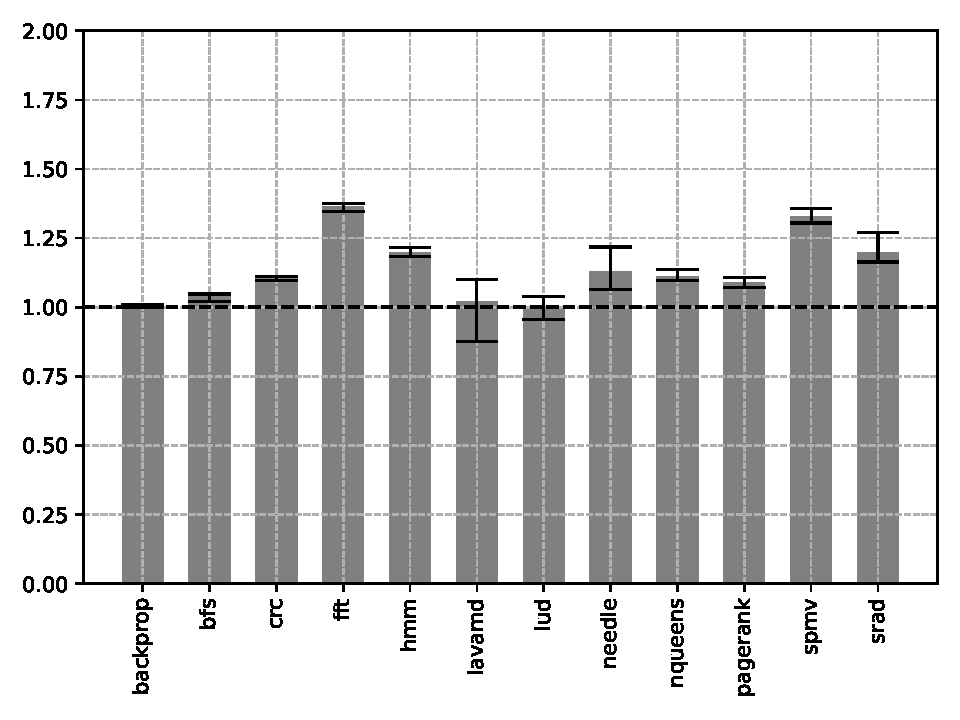
\includegraphics[width=\textwidth]
        {Images/6.1.RQ1/ostrich-wasmtime-opt.pdf}
        \caption{Ostrich}
    \end{subfigure}
    \begin{subfigure}[t]{.45\textwidth}
        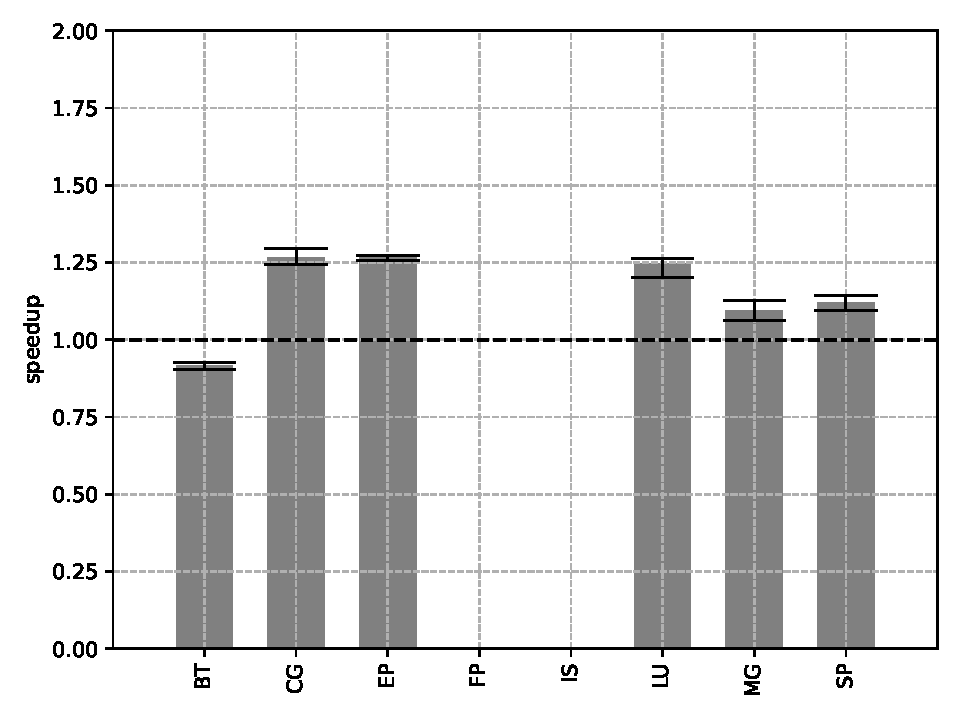
\includegraphics[width=\textwidth]
        {Images/6.1.RQ1/npb-wasmtime-opt.pdf}
        \caption{NPB}
    \end{subfigure}
    \caption{Bechmarks with optimized (\texttt{-O3}) on Wasmtime}
    \label{fig:rq1-wasmtime-opt}
\end{figure}

\begin{figure}
    \centering
    \begin{subfigure}[t]{\textwidth}
        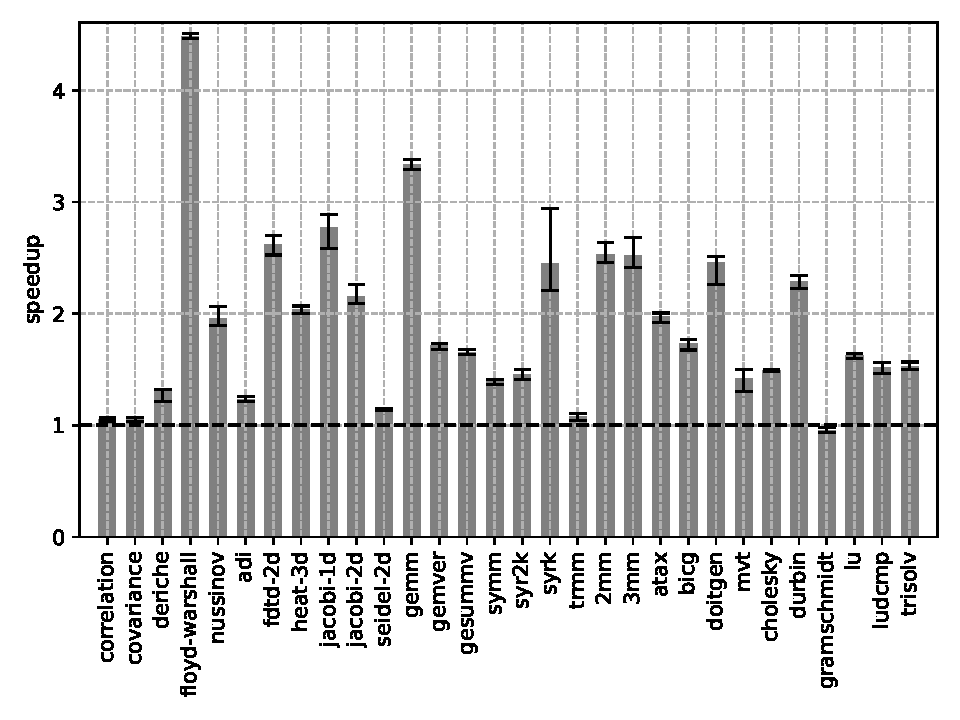
\includegraphics[width=\textwidth]
        {Images/6.1.RQ1/polybench-wasmer-cranelift-opt.pdf}
        \caption{Polybench}
    \end{subfigure}
    \begin{subfigure}[t]{.45\textwidth}
        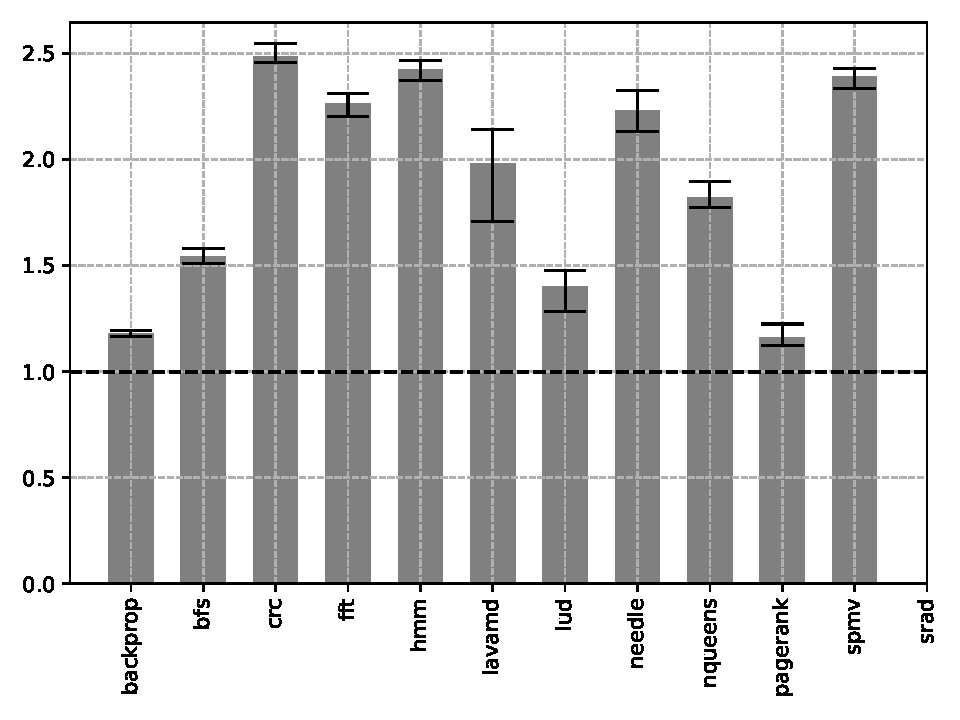
\includegraphics[width=\textwidth]
        {Images/6.1.RQ1/ostrich-wasmer-cranelift-opt.pdf}
        \caption{Ostrich}
    \end{subfigure}
    \begin{subfigure}[t]{.45\textwidth}
        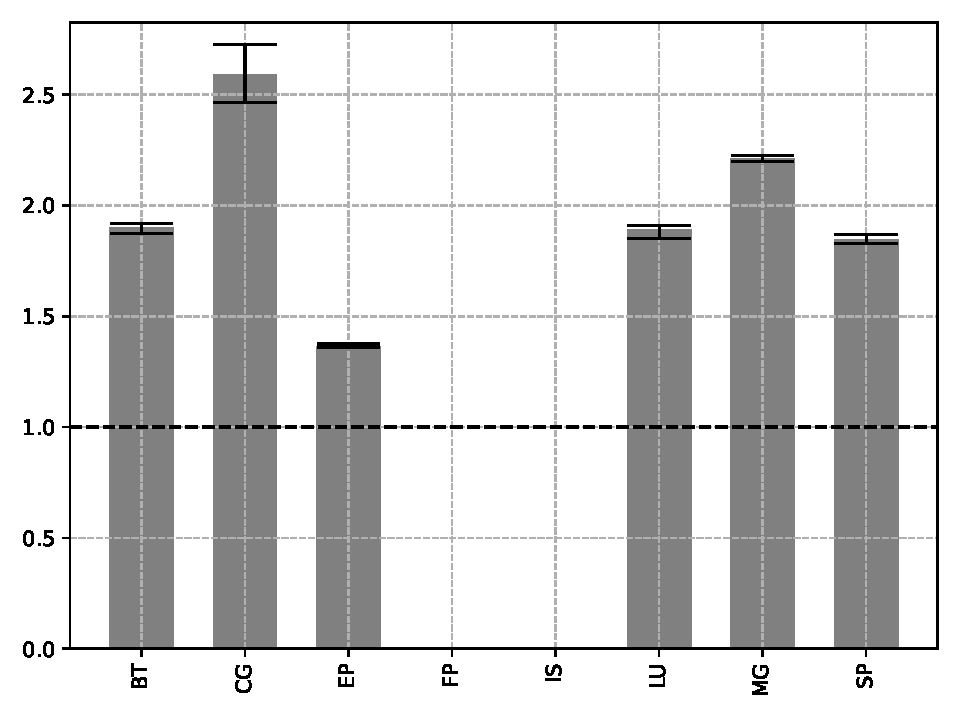
\includegraphics[width=\textwidth]
        {Images/6.1.RQ1/npb-wasmer-cranelift-opt.pdf}
        \caption{NPB}
    \end{subfigure}
    \caption{Bechmarks with optimized (\texttt{-O3}) on Wasmer(Cranelift)}
    \label{fig:rq1-wamer-cranelift-opt}
\end{figure}

\begin{figure}
    \centering
    \begin{subfigure}[t]{\textwidth}
        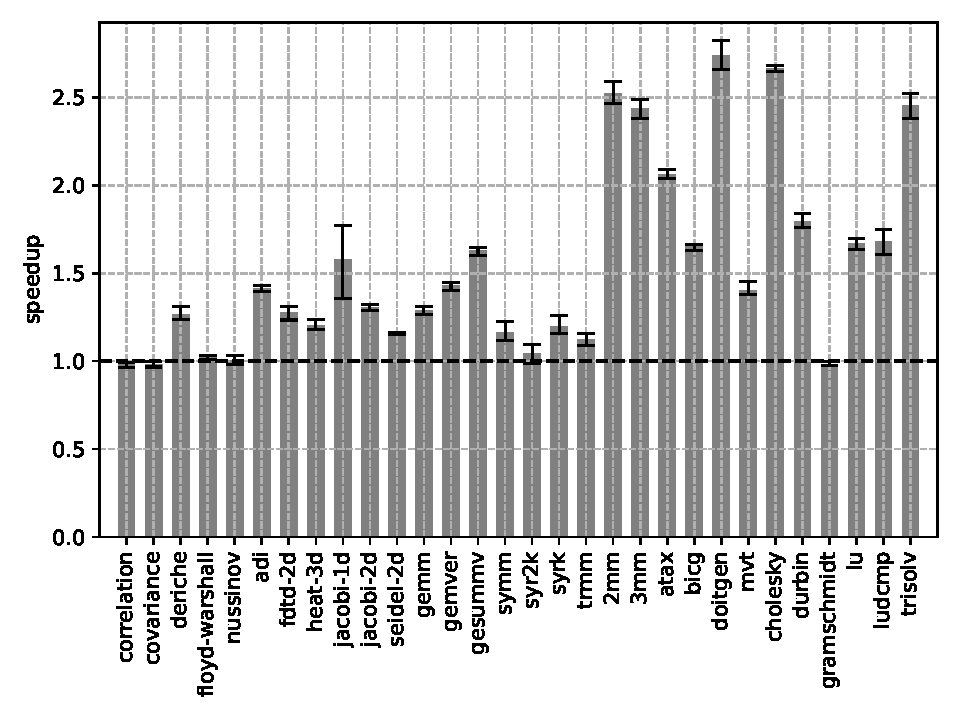
\includegraphics[width=\textwidth]
        {Images/6.1.RQ1/polybench-wasmer-llvm-opt.pdf}
        \caption{Polybench}
    \end{subfigure}
    \begin{subfigure}[t]{.45\textwidth}
        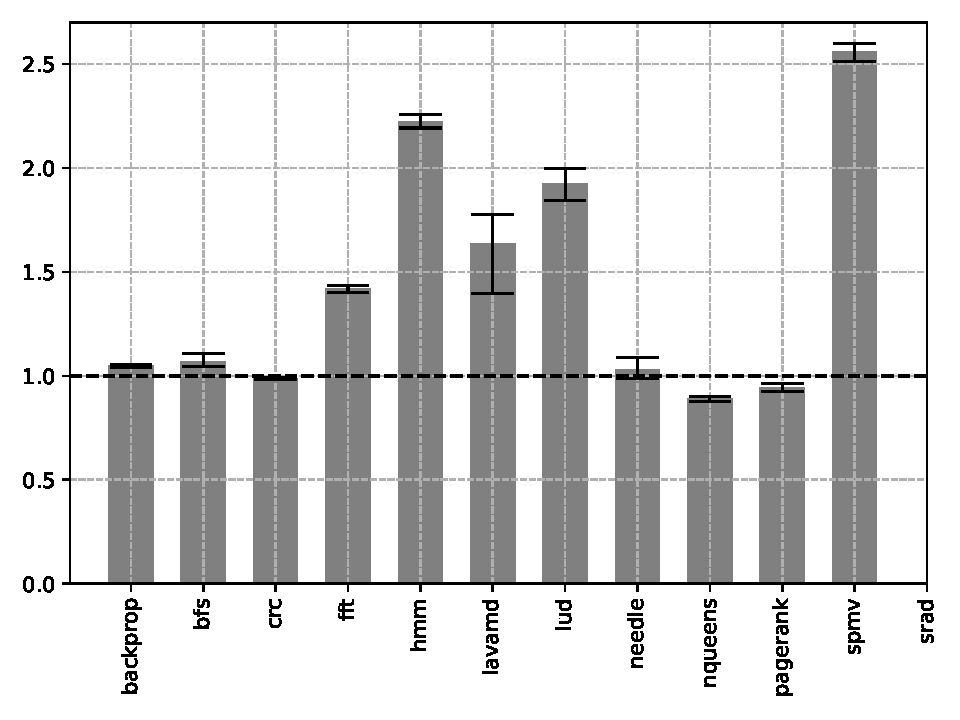
\includegraphics[width=\textwidth]
        {Images/6.1.RQ1/ostrich-wasmer-llvm-opt.pdf}
        \caption{Ostrich}
    \end{subfigure}
    \begin{subfigure}[t]{.45\textwidth}
        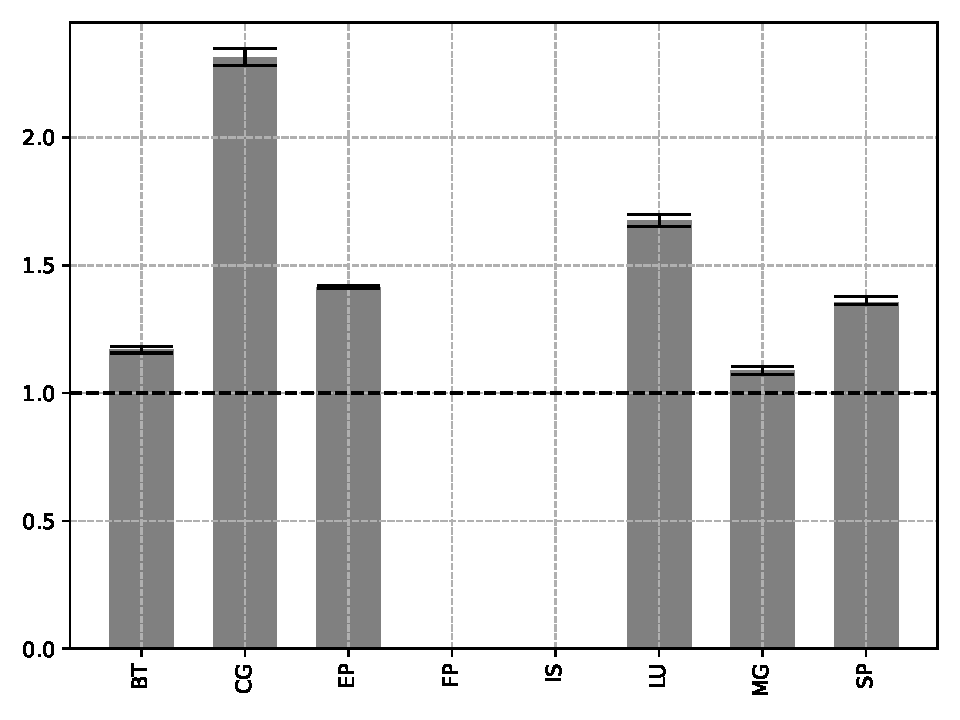
\includegraphics[width=\textwidth]
        {Images/6.1.RQ1/npb-wasmer-llvm-opt.pdf}
        \caption{NPB}
    \end{subfigure}
    \caption{Bechmarks with optimized (\texttt{-O3}) on Wasmer(LLVM)}
    \label{fig:rq1-wasmer-llvm-opt}
\end{figure}

\begin{figure}
    \centering
    \begin{subfigure}[t]{\textwidth}
        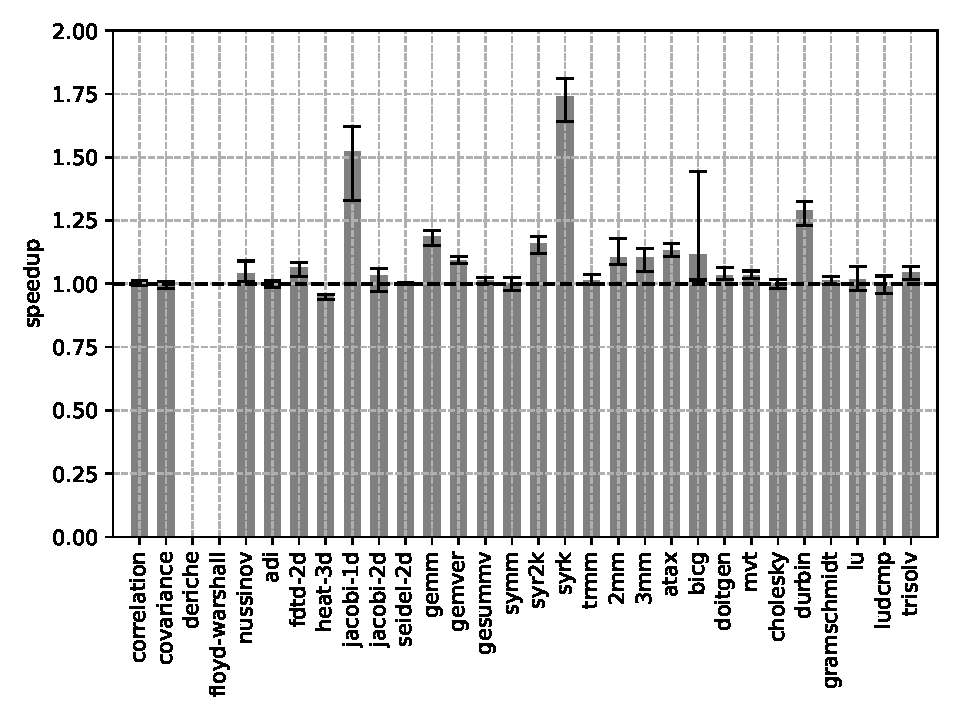
\includegraphics[width=\textwidth]
        {Images/6.1.RQ1/polybench-wasmtime-simd.pdf}
        \caption{Polybench}
    \end{subfigure}
    \begin{subfigure}[t]{.45\textwidth}
        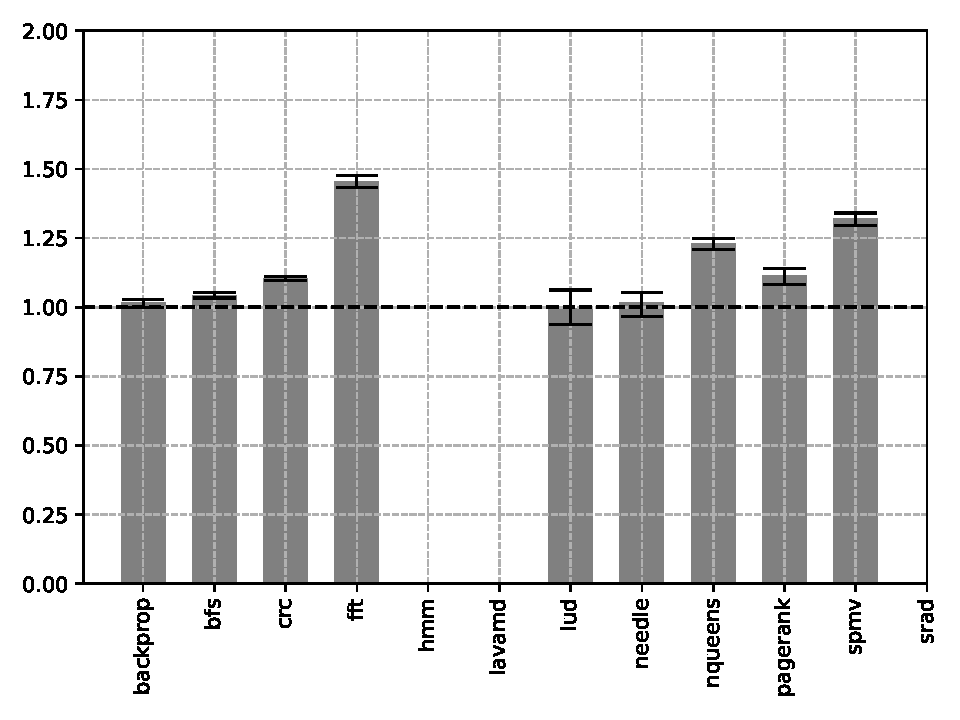
\includegraphics[width=\textwidth]
        {Images/6.1.RQ1/ostrich-wasmtime-simd.pdf}
        \caption{Ostrich}
    \end{subfigure}
    \begin{subfigure}[t]{.45\textwidth}
        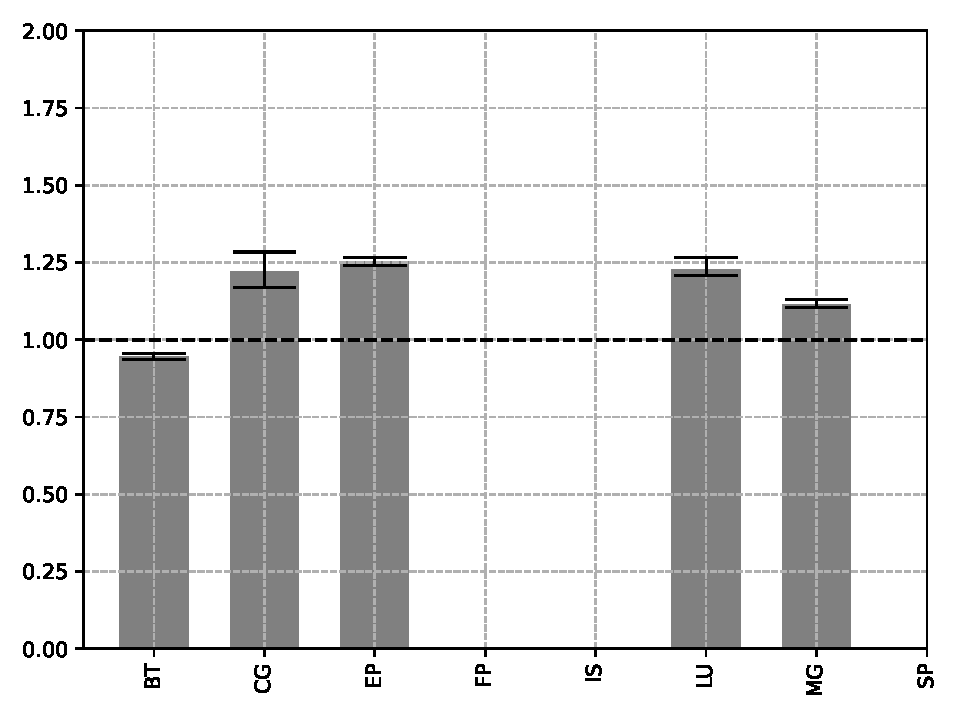
\includegraphics[width=\textwidth]
        {Images/6.1.RQ1/npb-wasmtime-simd.pdf}
        \caption{NPB}
    \end{subfigure}
    \caption{Bechmarks with SIMD extension (\texttt{-O3 -msimd128}) on Wasmtime}
    \label{fig:rq1-wasmtime-simd}
\end{figure}

\begin{figure}
    \centering
    \begin{subfigure}[t]{\textwidth}
        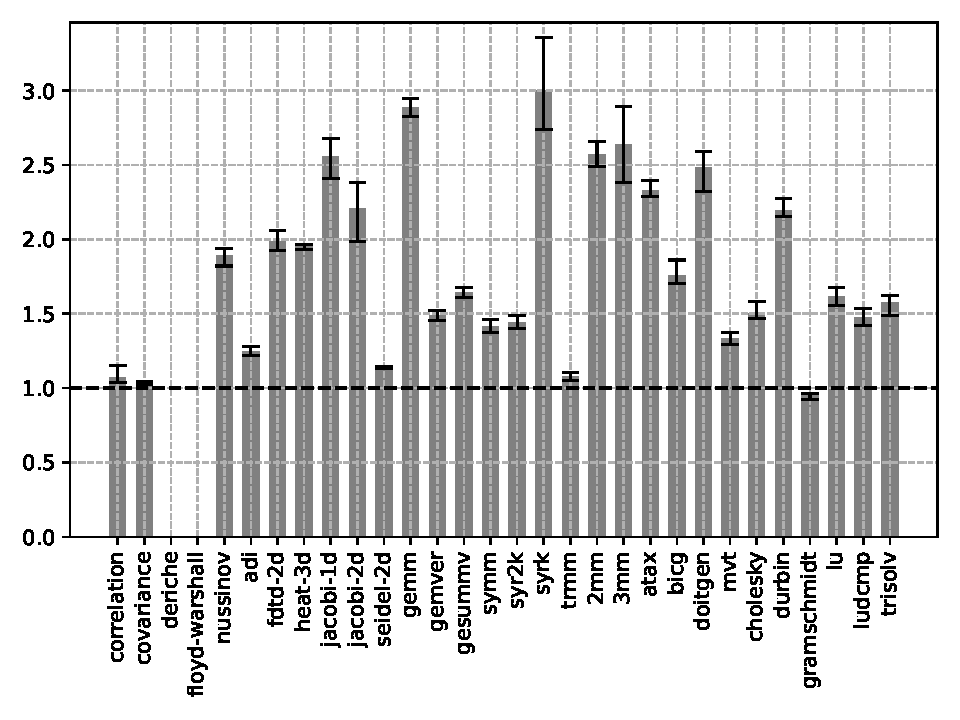
\includegraphics[width=\textwidth]
        {Images/6.1.RQ1/polybench-wasmer-cranelift-simd.pdf}
        \caption{Polybench}
    \end{subfigure}
    \begin{subfigure}[t]{.45\textwidth}
        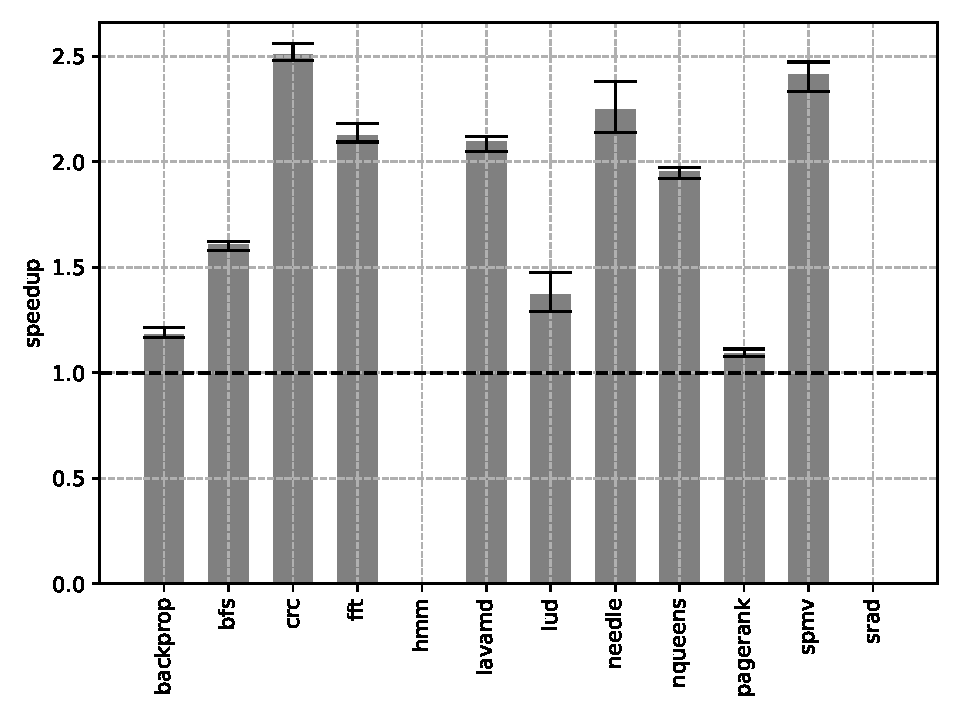
\includegraphics[width=\textwidth]
        {Images/6.1.RQ1/ostrich-wasmer-cranelift-simd.pdf}
        \caption{Ostrich}
    \end{subfigure}
    \begin{subfigure}[t]{.45\textwidth}
        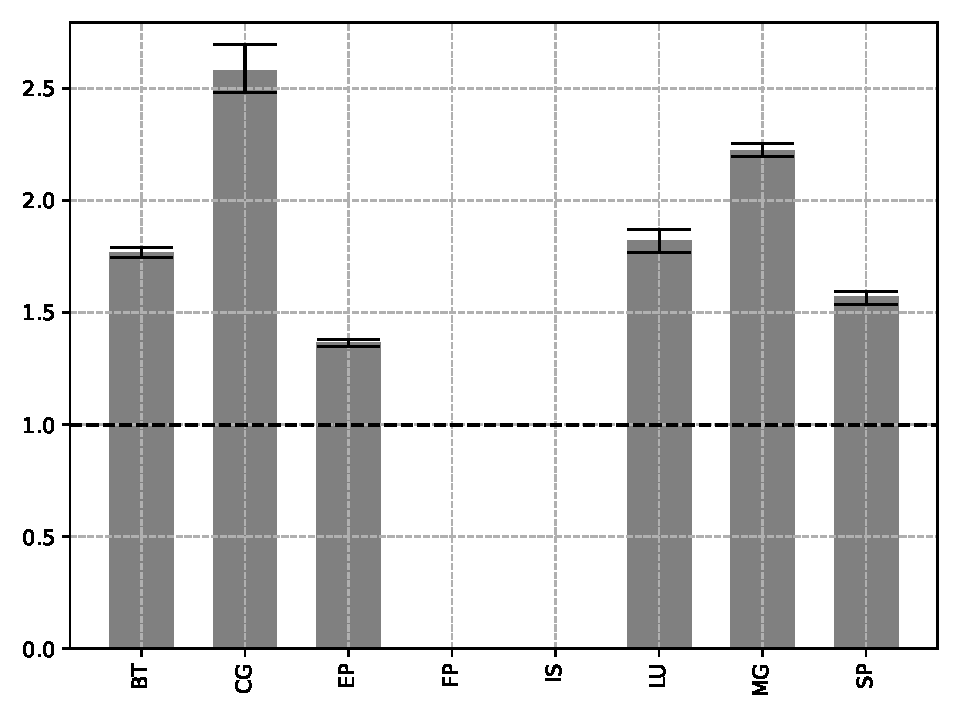
\includegraphics[width=\textwidth]
        {Images/6.1.RQ1/npb-wasmer-cranelift-simd.pdf}
        \caption{NPB}
    \end{subfigure}
    \caption{Bechmarks with SIMD extension (\texttt{-O3 -msimd128}) on Wasmer(Cranelift)}
    \label{fig:rq1-wasmer-cranelift-simd}
\end{figure}

\begin{figure}
    \centering
    \begin{subfigure}[t]{\textwidth}
        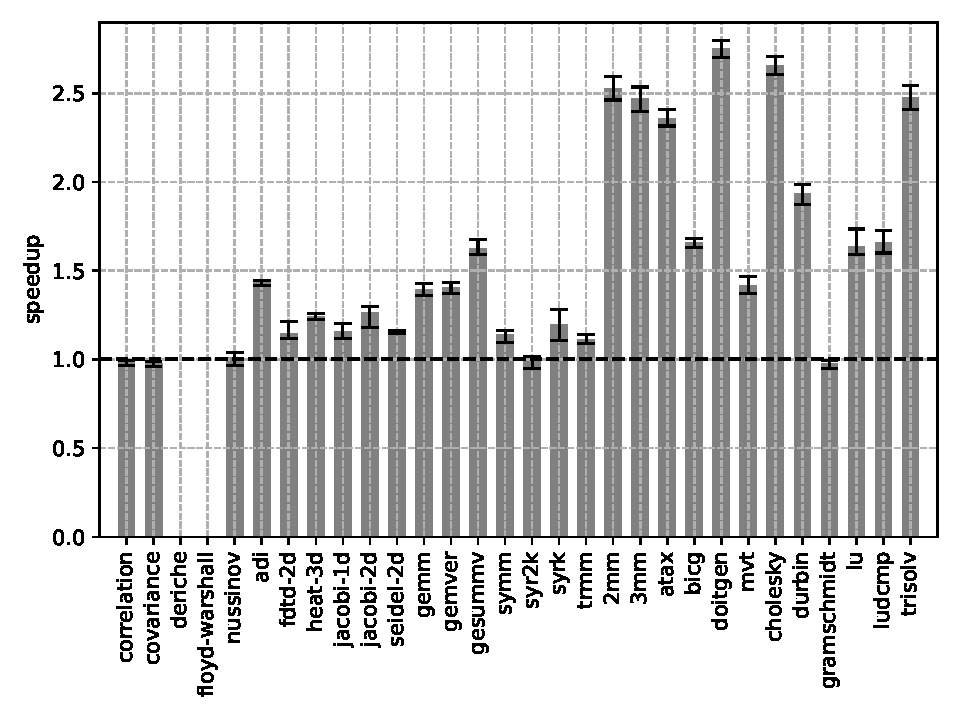
\includegraphics[width=\textwidth]
        {Images/6.1.RQ1/polybench-wasmer-llvm-simd.pdf}
        \caption{Polybench}
    \end{subfigure}
    \begin{subfigure}[t]{.45\textwidth}
        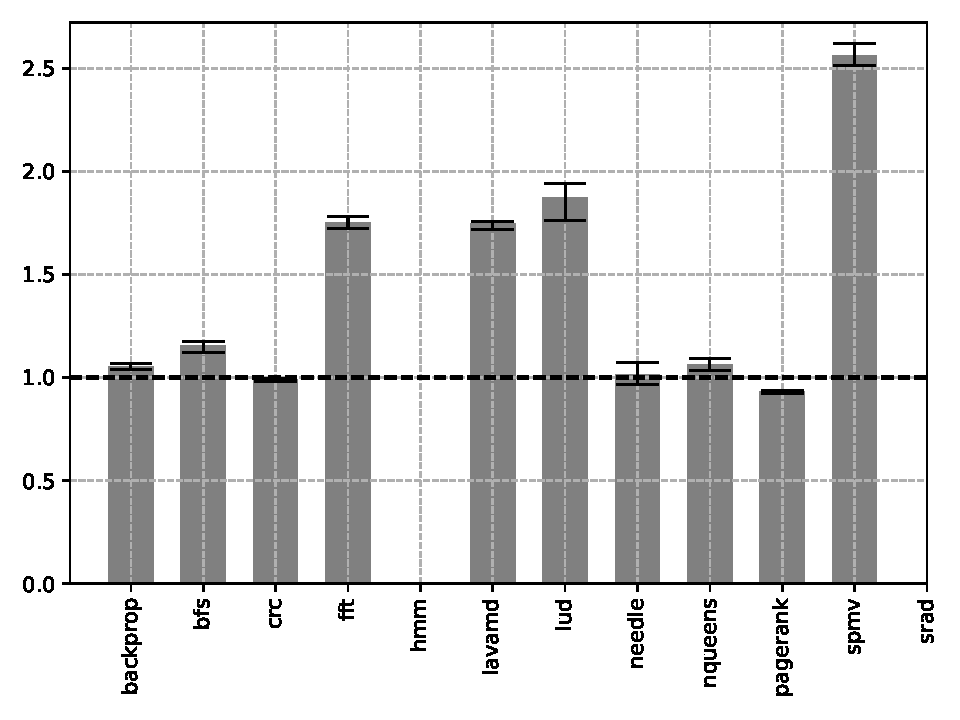
\includegraphics[width=\textwidth]
        {Images/6.1.RQ1/ostrich-wasmer-llvm-simd.pdf}
        \caption{Ostrich}
    \end{subfigure}
    \begin{subfigure}[t]{.45\textwidth}
        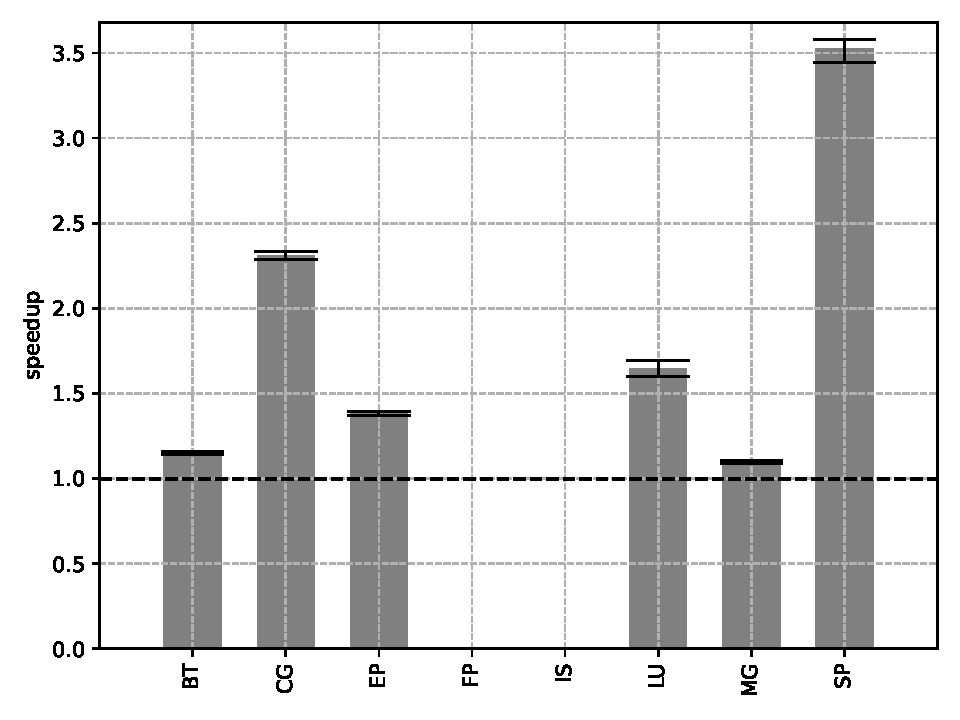
\includegraphics[width=\textwidth]
        {Images/6.1.RQ1/npb-wasmer-llvm-simd.pdf}
        \caption{NPB}
    \end{subfigure}
    \caption{Bechmarks with SIMD extension (\texttt{-O3 -msimd128}) on Wasmer(LLVM)}
    \label{fig:rq1-wasmer-llvm-simd}
\end{figure}

This section will compare SableWasm performance against several other WebAssembly runtime environments, specifically Wasmtime and Wasmer. We will benchmark three implementations over naive (\texttt{-O0}), optimized (\texttt{-O3}), and SIMD-enabled optimized (\texttt{-O3 -msimd128}) WebAssembly modules compiled from the source. One can consider Wasmtime \footnote{Wasmtime: \url{https://github.com/bytecodealliance/wasmtime}} as the `reference' implementation of WebAssembly out of the browser and maintained by the WebAssembly community group. The system is built upon the  custom compile framework, Cranelift \footnote{Cranelift: \url{https://github.com/bytecodealliance/wasmtime/tree/main/cranelift}}. Currently, both Cranelift and Wasmtime are still under active development and subject to changes in the future. Here, in this project, we anchor our Wasmtime at version 0.26.0. Wasmer \footnote{Wasmer: \url{https://wasmer.io/}} is another community approach for running WebAssembly sandboxed applications outside of the browser. It comes with a package manager, WAPM \footnote{WAPM: \url{https://wapm.io/}}, that distributes applications in WebAssembly binary module format. Wasmer supports three compiler backends, LLVM, Cranelift, and a one-pass code generator for fast compilation. In this chapter, we will focus on the LLVM and Cranelift variants of Wasmer. Similar to Wasmtime, Wasmer is also under active development at the time of thesis writing, and we fix the version of Wasmer at 1.0.2. Unlike SableWasm, an ahead-of-time(AOT) compiler for WebAssembly modules, Wasmtime and Wasmer are both just-in-time (JIT). Thus, when measuring the benchmark's performance, we need to isolate the error induced by the compiler, such as compilation-overhead and warm-up time. To eliminate the compilation-overhead, we measure the execution time within the internal timing code by issuing syscalls to the WASI layer. Further, we adjust the benchmark size for Ostrich and NPB so that each benchmark case takes more than 10 seconds to compute to reduce the error introduced by the JIT warm-up process.

Figure~\ref{fig:rq1-wasmtime-naive} to figure~\ref{fig:rq1-wasmer-llvm-simd} presents the benchmark result. We normalize the data with respect to the SableWasm's execution time and present them as speed-ups. A number higher than one means that the SableWasm's performance is better than the candidate, and on the other hand, a less than one speed-up refers to slow-down. The error bar is calculated based on the  10th percentile and 90th percentile accordingly. For naive translated WebAssembly modules, SableWasm performs better than Wasmtime in most benchmark cases but slower in seven cases in total.

For naive translated WebAssembly modules, SableWasm performs better than Wasmtime in most benchmark cases except seven of them. We suspect that slow down comes from the excessive linear memory access. In the current version of the WASI-enable Clang compiler, a naive translated module will use linear memory to simulate stack frame functions instead of using local variables. This means that when writing to a function local variable, SableWasm needs to first load the linear memory base pointer from the instance object, calculate the address and then perform the memory access. Making the case worse, the current SableWasm will always load the base memory pointer even if a local variable already holds the base pointer. LLVM cannot effectively eliminate these load instructions, as the linear memory base pointer in the instance object is volatile. One possible solution to ease the problem is to carefully annotate the instance object pointer so that the alias analysis in SableWasm can correctly identify these redundant load instructions. On the other hand, SableWasm performs better than Wasmer with both Cranelift or LLVM backend. This is quite interesting as the current SableWasm is also built upon LLVM. We suspect that two factors are contributing to the speedup. First, SableWasm employs several optimization techniques to improve the quality of the generated LLVM intermediate representation. When designing the translation patterns for lowering SableWasm MIR into LLVM IR, we notice that the quality of LLVM IR has a significant impact on the result performance, especially for auto-vectorization. Second, Wasmer supports many other safety features that are not specified in the WebAssembly specification, such as stack probing. These safety features impose performance drawbacks on the system and can be observed from the benchmark results above.

For optimized and SIMD-enabled input WebAssembly modules, SableWasm performs on par with Wasmtime, except on benchmark case \texttt{durbin}. One may also notice that the error for \texttt{durbin} in figure~\ref{fig:rq1-wasmtime-opt-polybench} is more significant compared to others. This is due to the nature of \texttt{durbin} benchmark case. For Ostrich and NPB, we can adjust the benchmark size to reduce the measurement errors. However, this is not the case for Polybench, as the input size is hardcoded. On the other hand, SableWasm performs better than Wasmer in most of the benchmark cases. Here we will take \texttt{floyd-warshall} as an example. The core computation function in \texttt{floyd-warshall} is a nested for loop that iteratively multiplies then adds matrices. This operation is highly parallel. We notice that the performance of SableWasm is approximately four times better in optimized input and two times better for SIMD-enabled. Currently, there seems no way to retrieve generated LLVM IR from Wasmer, and we can only suspect reasons based on the experiment result. We suspect that the auto-vectorization may cause this in the LLVM framework. The four times and two times speedup appears to align with the SIMD vector operations for packed double-precision floating-point numbers. Thus, Wasmer may contain awkwardly generated LLVM intermediate representation that stops auto-vectorization pass to turn scalar code into the vectorized form.

\begin{table}[]
    \centering
    % Please add the following required packages to your document preamble:
% \usepackage{multirow}
% \usepackage[table,xcdraw]{xcolor}
% If you use beamer only pass "xcolor=table" option, i.e. \documentclass[xcolor=table]{beamer}

\begin{tabular}{ll|ccc}
    \multicolumn{2}{c|}{\textbf{Benchmark name}}                 & \textbf{Wasmtime}                   & \textbf{Wasmer (Cranelift)} & \textbf{Wasmer (LLVM)}                                    \\ \hline
    \rowcolor[HTML]{C0C0C0}
    \cellcolor[HTML]{C0C0C0}                                     & Naive                               & 1.19                        & 3.18                        & 1.50                        \\
    \rowcolor[HTML]{C0C0C0}
    \cellcolor[HTML]{C0C0C0}                                     & Optimized                           & 1.09                        & 1.90                        & 1.54                        \\
    \rowcolor[HTML]{C0C0C0}
    \multirow{-3}{*}{\cellcolor[HTML]{C0C0C0}\textbf{Polybench}} & SIMD-enabled                        & 1.10                        & 1.80                        & 1.56                        \\ \hline
                                                                 & Naive                               & 1.07                        & 2.43                        & 1.34                        \\
                                                                 & Optimized                           & 1.13                        & 1.90                        & 1.43                        \\
    \multirow{-3}{*}{\textbf{Ostrich}}                           & SIMD-enabled                        & 1.14                        & 1.86                        & 1.41                        \\ \hline
    \rowcolor[HTML]{C0C0C0}
    \cellcolor[HTML]{C0C0C0}                                     & {\color[HTML]{333333} Naive}        & {\color[HTML]{333333} 1.23} & {\color[HTML]{333333} 3.42} & {\color[HTML]{333333} 1.86} \\
    \rowcolor[HTML]{C0C0C0}
    \cellcolor[HTML]{C0C0C0}                                     & {\color[HTML]{333333} Optimized}    & {\color[HTML]{333333} 1.15} & {\color[HTML]{333333} 1.97} & {\color[HTML]{333333} 1.50} \\
    \rowcolor[HTML]{C0C0C0}
    \multirow{-3}{*}{\cellcolor[HTML]{C0C0C0}\textbf{NPB}}       & {\color[HTML]{333333} SIMD-enabled} & {\color[HTML]{333333} 1.15} & {\color[HTML]{333333} 1.89} & {\color[HTML]{333333} 1.85}
\end{tabular}

    \caption{Average speedups compare to Wasmtime and Wasmer}
    \label{tbl:rq1-average}
\end{table}

In general, we conclude that SableWasm performs on par with Wasmtime on optimized and SIMD-enabled WebAssembly modules and better than Wasmtime and Wasmer for other benchmark cases, as shown in table~\ref{tbl:rq1-average}.


\section[RQ2: Does optimization over input modules matter?]{
  {\large RQ2: Does optimization over input modules matter?}}

\section[RQ3: How much does SIMD extension improve in performance?]{
  {\large RQ3: How much does SIMD extension improve in performance?}}